\clearpage{\pagestyle{empty}\cleardoublepage}
\chapter{Block RAM}


Mentre nel nostro progetto per semplicit\`a  abbiamo considerato nulli i tempi d'accesso alla cache e alla memoria principale, ovviamente ci\`o non accade nella realt\`a dove la struttura gerarchica delle memorie impone vincoli di dimensione e tempi d'accesso per i vari livelli di memoria. Per tale motivo abbiamo voluto approfondire le problematiche relative alle temporizzazioni per gli accessi in memoria che un progetto tradizionale impone. Per far ci\`o abbiamo considerato ci\`o che una tipica FPGA d\`a a disposizione ad un progettista per implementare una memoria ram e gestirne gli accessi in lettura e scrittura.
\\
Nel nostro caso abbiamo analizzato le caratteristiche dell'FPGA della famiglia Spartan-3E di Xilinx, che per gestire la memorizzazione di dati utilizza le Block Ram.

\section{Caratteristiche e segnali della Block Ram}

La memoria RAM presente su una FPGA Spartan-3 viene implementata tramite una serie di Block Ram ripartite in colonne il cui numero e capacit\`a dipende dalle caratteristiche stesse della scheda utilizzata. Dal punto di vista implementativo le Block Ram sono realizzate tramite 18,432 celle di memoria SRAM che consentono pertanto di memorizzare 18 Kbits di cui 16 Kbits di dato e 2 Kbits utilizzati tipicamente per memorizzare i bit di parit\`a relativi ai dati memorizzati o in alternativa come spazio di memorizzazione aggiuntivo.\\
L'accesso alla block ram pu\`o avvenire o in modalit\`a Single-Port utilizzando una sola porta dati (A o B) oppure in Dual-Port  tramite 2 porte indipendenti A e B che consentono di effettuare operazioni di lettura e scrittura su zone diverse del dispositivo.

\begin{figure}[!h]
\centering
% 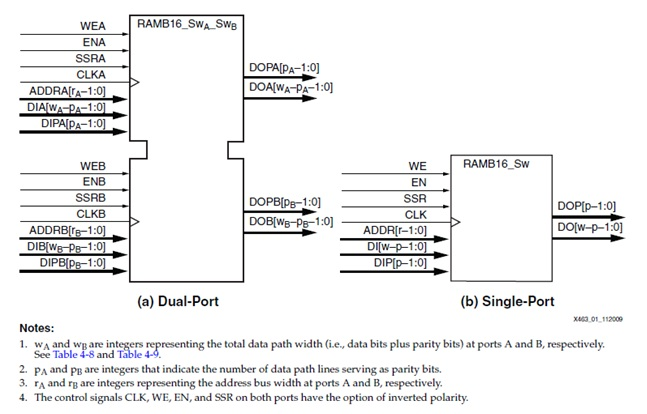
\includegraphics[scale=0.8]{img/blockRam/pinoutPorte.jpg}
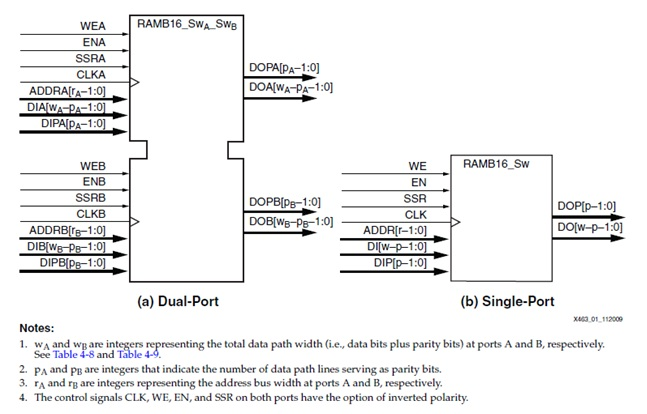
\includegraphics[width=\textwidth]{img/blockRam/pinoutPorte.jpg}
\caption{Pinout Block Ram Single-Port e Dual-Port}
\label{fig:set_ass}
\end{figure}


Ogni  porta della block ram si interfaccia con due bus dati (distinti per l'input e per l'output),  con il bus degli indirizzi e dispone di una serie di segnali di comando atti ad abilitare il dispositivo (EN in Single-Port) e a gestire operazioni di lettura (EN) o scrittura (WE). La seguente tabella racchiude i principali segnali illustrati nella figura precedente sia in Single-Port che in Dual-Port.

\begin{figure}[!h]
\centering
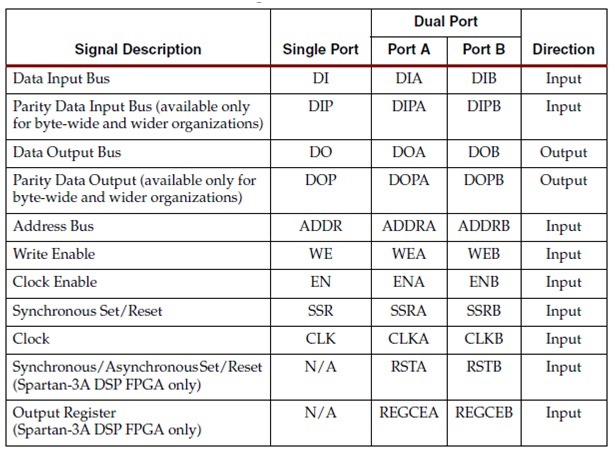
\includegraphics[width=\textwidth]{img/blockRam/segnali.jpg}
\caption{Segnali della Block Ram Single-Port e Dual-Port}
\label{fig:set_ass}
\end{figure}

Segnali di comando:

\begin{itemize}
  \item \texttt{EN} = Enable consente di abilitare il dispositivo e qualora non siano asseriti WE(write enable) o SSR (reset), il 	segnale comanda a default la lettura della cella di memoria all'indirizzo specificato sul bus degli indirizzi ADDR sul 		fronte positivo del clock.
  \item \texttt{WE} = Write Enable consente di comandare un ciclo di scrittura in memoria all'indirizzo specificato sul bus degli indirizzi ADDR (con EN asserito), tale operazione in base al valore settato nell'attributo WRITE\_MODE pu\`o essere affiancata da una lettura contemporanea del dato alla stessa locazione di memoria che viene portato nel buffer di output sul bus DO (della stessa porta). 
  \item \texttt{SSR} = Syncronous Set/Reset consente di settare '1' o resettare '0' i registri di ouput sul bus dati in accordo col valore dell'attributo SRVAL.
  \item \texttt{REGCE} = Output Register Enable consente in fase di  lettura da ram di salvare il dato letto in un output register.
  \item \texttt{CLK} =  \`e il clock e si pu\`o configurare se la memoria debba essere sensibile ai fronti di salita o di discesa.
\item \texttt{GSR} = Global Set/Reset segnale di sistema utilizzato per in fase di inizializzazione del sistema (non disponibile all'esterno su un pin).
\end{itemize}

C'\'e inoltre la possibilit\`a di configurare le polarit\`a di ogni segnale di comando se da considerarsi asserito alto o basso.
\\
Interfacciamento ai bus:\\

\begin{itemize}
  \item \texttt{ADDR} = bus degli indirizzi la cui larghezza [\#:0] dipende dalla configurazione della block ram.
  \item \texttt{DI} = Data Input Bus [\#:0] (l'ampiezza del dato da trasferire dipende dalla configurazione della block ram).
  \item \texttt{DO} = Data Output Bus
  \item \texttt{DIP} = Data Input Parity Bus (nei bit pi\`u significative del Bus Dati di Input)
  \item \texttt{DOP} = Data Output Parity Bus (nei bit pi\`u significative del Bus Dati di Output)
\end{itemize}

Possibili configurazioni e organizzazioni della Block Ram:\\

\begin{figure}[!h]
\centering
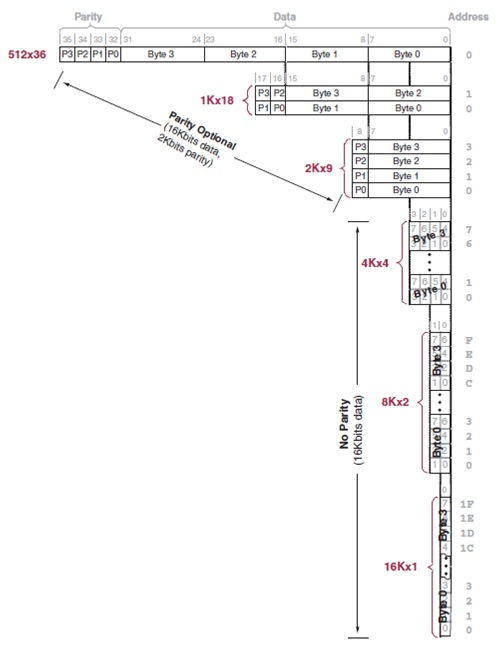
\includegraphics[width=\textwidth]{img/blockRam/organInterna.jpg}
\caption{Possibili organizzazioni interne della Block Ram}
\label{fig:set_ass}
\end{figure}

Nel nostro caso, dal momento che il DLX \`e un processore a 32 bit, la configurazione necessaria per la block ram \`e la 512x36. Tale configurazione da la possibilit\'a di accedere fino a 36 bit di dato contemporaneamente, di cui 32 bit di dato veri e 4 di parit\`a posti sui bit pi\`u significativi del bus dati. Con tale configurazione la block ram (di 18 Kbit) conterr\`a 512 entry (memory-depth) da 36 bit (infatti 512x36 bit = 18 Kbits).

\section{Configurazione della Block Ram}

La configurazione della Block Ram avviene tramite una serie di attributi propri dei componenti ram disponibili nelle librerie di sistema tramite i quali si pu\`o settare in base alle specifiche di progetto l'organizzazione interna, la dimensione e diverse altre modalità di funzionamento che la Block Ram offre all'utente.\\
Generalmente il numero di porte della ram e la sua organizzazione interna possono essere specificati utilizzando Xilinx Core Generator che consente di configurare tramite un wizard la Block Ram ottenendo direttamente il codice VHDL del componente ram desiderato oppure si possono utilizzare i tipi VHDL  gi\`a associati alla Block Ram RAMB16\_Sn dove n corrisponde all'ampiezza del dato + parit\`a.

\begin{figure}[!h]
\centering
%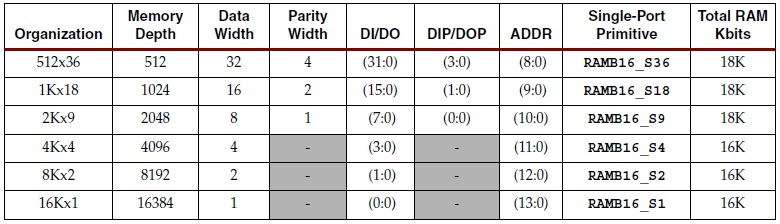
\includegraphics[width=\textwidth]{img/blockRam/tabTipiRam.jpg}
 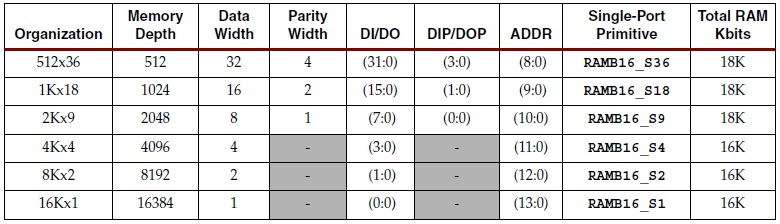
\includegraphics[scale=0.5]{img/blockRam/tabTipiRam.jpg}
\caption{La tabella mostra le diverse tipologie di RAMB\_Sn ottenibili dalla Block Ram in base all'organizzazione interna desiderata}
\label{fig:set_ass}
\end{figure}

\begin{itemize}
  \item \texttt{INIT\_xx - INITP\_xx}
A default la block ram \`e inizializzata a tutti 0, ma \`e possibile in inizializzarne il contenuto in diversi modi o direttamente tramite Core Generator al momento della configurazione del componente oppure tramite opportuni attributi VHDL come INIT\_xx e INITP\_xx (per inizializzare i bit di parit\`a). 
Nel primo caso si passa direttamente un file di coefficienti (.coe) che definisce in primo luogo la base numerica dei dati da inserire e in seguito l'elenco dei dati elencati a partire dalla parte bassa della memoria fino agli indirizzi alti. Un esempio della struttura di tale file \`e il seguente:\\\\
	memory\_inizialization\_radix=16;\\
	memory\_inizialization\_vector=80, 0F, 00, 0B, ..., 82;\\

Altrimenti si utilizzano direttamente 64 attributi VHDL INIT\_xx (da INIT\_00 a INIT\_3F) che consentono di inizializzare le 64 zone da 256bit con cui \`e ripartita la memoria. Gli indirizzi del blocco di memoria da inizializzare identificati da xx sono calcolabili nel seguente modo dopo aver convertito l'indirizzo esadecimale xx nel corrispondente indirizzo decimale yy:
\\
indirizzo iniziale del blocco xx = [(yy+1)*256] - 1
indirizzo finale del blocco xx = yy*256
\\
\begin{figure}[!h]
\centering
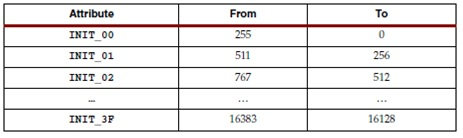
\includegraphics[width=\textwidth]{img/blockRam/init.jpg}
\caption{Attributi di Inizializzazione del contenuto della Block Ram}
\label{fig:set_ass}
\end{figure}

INITP\_xx sono attributi analoghi che consentono di inizializzare i bit di parit \`a presenti in memoria (da INITP\_00 a INITP\_07).
\item \texttt{INIT}  \`e l'attributo utilizzato in fase di inizializzazione per settare il valore iniziale del registro di output quando viene asserito il segnale GSR.
\\
\item \texttt{WRITE\_MODE}  \`e l'attributo che consente di settare il comportamento dei registri in output (relativamente ad una porta) che forniscono il dato sull'Output Data Bus durante un ciclo di scrittura in memoria.

\begin{enumerate}
\item \texttt{WRITE\_FIRST} \`e  il valore di default e comporta un comportamento Read after Write della memoria, ovvero durante un ciclo di scrittura il dato in input viene contemporaneamente scritto alla locazione di memoria indicata dall'indirizzo e portato nel registro di output. 
Nel caso di utilizzo in Dual-Port si ha l'invalidazione del contenuto del registro di output dell'altra porta.

\begin{figure}[!h]
\centering
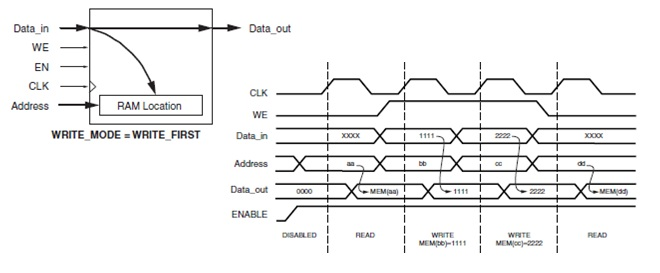
\includegraphics[width=\textwidth]{img/blockRam/writeFirst.jpg}
\label{fig:set_ass}
\end{figure}

\item \texttt{READ\_FIRST} determina un comportamento Read before Write, ovvero prima si carica nel buffer di output il dato (passato) presente alla locazione di memoria specificata dall'indirizzo e poi si sovrascrive tale zona di memoria col dato in ingresso (si effettua la scrittura in memoria). 

\begin{figure}[!h]
\centering
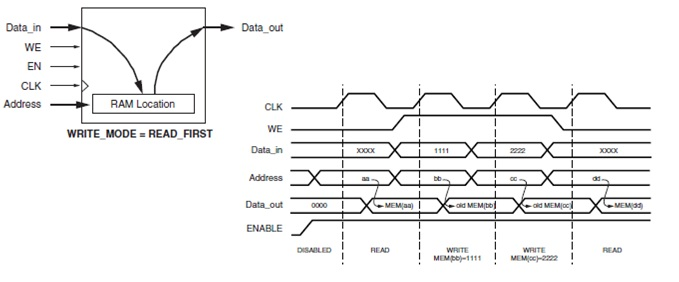
\includegraphics[width=\textwidth]{img/blockRam/readFirst.jpg}
\label{fig:set_ass}
\end{figure}

\item \texttt{NO\_CHANGE} determina un comportamento classico di scrittura in memoria senza alcun aggiornamento del dato contenuto nel registro in output. Nel caso di utilizzo in Dual-Port si ha come side-effect l'invalidazione del contenuto del registro di output dell'altra porta.
\end{enumerate}

\begin{figure}[!h]
\centering
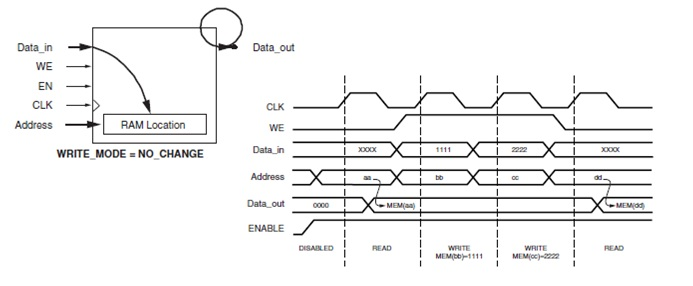
\includegraphics[width=\textwidth]{img/blockRam/noChange.jpg}
\label{fig:set_ass}
\end{figure}

\end{itemize}

\section{Operazioni della Block Ram}

Di seguito viene riportato l'elenco delle operazioni che la Block Ram  \`e in grado di gestire e dei relativi segnali impiegati:

\begin{itemize}
  \item Global Set/Reset: segue la fase di inizializzazione iniziale del contenuto della Block Ram in cui si inizializza la ram o a tutti zeri (default) o ai valori impostati con gli attributi \texttt{INIT\_xx}. Tale segnale serve per inizializzare lo stato dei flipflop e registri di output che vengono settati in base al valore specificato dall'attributo \texttt{INIT} (0 a default). 

\item RAM Disabled: se il segnale \texttt{EN} non  \`e asserito la ram mantiene il proprio stato. Ogni operazione prevede che EN venga asserito affinch\`e la ram sia attiva.

\item Synchronous Set/Reset: \`e l'operazione conseguente all'asserzione contemporanea dei segnali \texttt{EN} e \texttt{SSR}. Tale operazione comporta la re inizializzazione dei registri di output al valore specificato dall'attributo\texttt{ SRVAL}.

\item \texttt{WE} + \texttt{SSR} comporta un ciclo di scrittura in cui il dato in input viene salvato in memoria all'indirizzo presente sul bus degli indirizzi, mentre il registro di output viene impostate al valore SRVAL.

\item READ: la lettura sulla block ram avviene in modo sincrono, quindi sul fronte positivo del clock qualora sia asserito il solo segnale di \texttt{EN}.

\item WRITE: la scrittura sulla block ram avviene in modo sincrono sul fronte positivo del clock e qualora siano asseriti contemporaneamente \texttt{EN} + \texttt{WE}. La scrittura del dato in input sui pin dell'Input Data Bus avviene all'indirizzo specificato e tale operazione  \`e affiancata contemporaneamente dalla lettura del dato alla stessa locazione di memoria che viene reso disponibile in lettura e caricato sui registri di output (naturalmente la politica con la quale avviene tale operazione di scrittura e lettura simultanea  \`e definita dal valore dell'attributo WRITE\_MODE visto in precedenza).
\end{itemize}

La seguente tabella racchiude quanto detto in precedenza e associa ad ogni operazione i valori dei segnali associati.

\begin{figure}[!h]
\centering
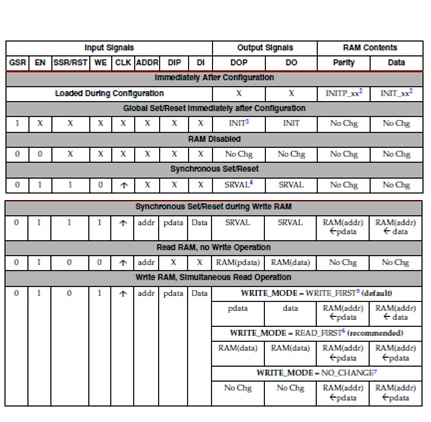
\includegraphics[width=\textwidth]{img/blockRam/operazioni.jpg}
\label{fig:set_ass}
\end{figure}

\section{Conflitti d'accesso in Block Ram Dual-Port}
Utilizzando la block ram in modalit\`a Dual-Port  si ha la possibilit\`a di utilizzare contemporaneamente le due porte per accedere alla memoria sia in lettura e scrittura e mentre da un lato ci\`o consente di aumentare lo throughput complessivo dei dati trasferiti, dall'altro vi sono potenziali problemi di conflitto negli accessi simultanei alle stesse celle di memoria.
\\
Le condizioni di potenziale conflitto si hanno nei seguenti casi:

\begin{enumerate}
	\item Scrittura simultanea sulle due porte alla stessa locazione di memoria.\\
	Tale situazione non ha un meccanismo di arbitraggio per far fronte ad accessi in scrittura simultanei, ma l'effetto prodotto è quello di comportare l'invalidazione del contenuto dell'area di memoria coinvolta.
	\item Conflitti per temporizzazioni clock-to-clock tra le due porte.\\
Ci\`o accade a causa dei clock diversi che comandano le operazioni tra le due porte che sono troppo ravvicinati tra loro e il clock della porta in lettura non rispetta i tempi di setup per l'accesso in scrittura al dispositivo (arriva troppo presto quando ancora non la scrittura in memoria non ha terminato). Un esempio \`e il seguente:

\begin{figure}[!h]
\centering
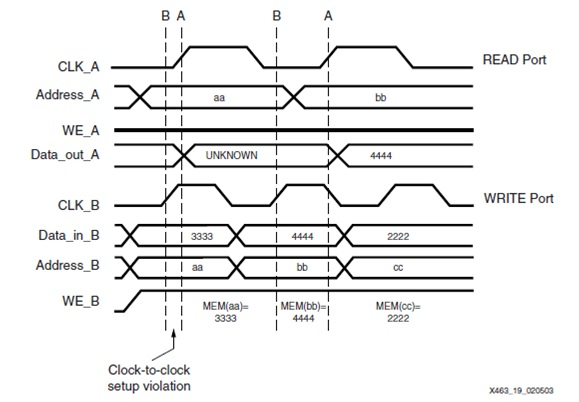
\includegraphics[width=\textwidth]{img/blockRam/conflittiTemp.jpg}
\label{fig:set_ass}
\end{figure} 

Nel primo caso, la porta B inizia la scrittura in memoria all'indirizzo aa del dato 3333 e poco dopo, prima che la scrittura abbia terminato, arriva il fronte del CLK\_A che fa iniziare la lettura allo stesso indirizzo aa violando il tempo di setup necessario per scrivere il dato in memoria. Nel secondo caso invece si ha la scrittura da parte della porta B all'indirizzo bb del dato 4444 e in questo caso CLK\_A rispetta le temporizzazioni di scrittura e la porta A legge il dato correttamente scritto in memoria.

	\item Scrittura e Lettura contemporanea sulla stessa zona di memoria in funzione del WRITE\_MODE impostato.\\
Nei casi di scrittura su una porta e lettura sull'altra, se si utilizza WRITE\_MODE= NO\_CHANGE o WRITE\_FIRST, la scrittura su una porta invalida automaticamente il contenuto del registro di output (in lettura) dell'altra porta, per tale motivo  \`e consigliabile la modalit \`a di scrittura READ\_FIRST per evitare conflitti sulla porta in lettura.

\begin{figure}[!h]
\centering
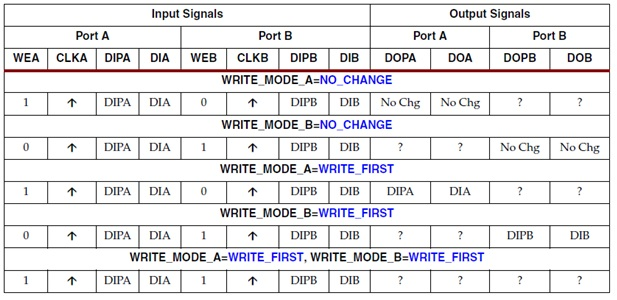
\includegraphics[width=\textwidth]{img/blockRam/conflittiScritture.jpg}
\label{fig:set_ass}
\end{figure}

\end{enumerate}

Per semplicit\`a implementativa la Block Ram non implementa un sistema di arbitraggio per gestire tali conflitti che sono lasciati a cura del progettista e comunque in caso di conflitto dovuto a scritture contemporanee non si verificano danni fisici al dispositivo di memoria. 

\section{Possibili utilizzai della Block Ram in un progetto su FPGA}
La Block Ram pu\`o essere utilizzata in un progetto su FPGA per implementare una serie di funzionalit\`a che coinvolgano la memorizzazione di dati. I principali possibili utilizzi sono i seguenti:
\begin{enumerate}
\item RAM utilizzata da un microprocessore integrato sull'FPGA per memorizzare dati accessibili in lettura e scrittura.
\item ROM realizzata attraverso l'inizializzazione del suo contenuto all'avvio del sistema e accessibile in sola lettura.
\item Memorie FIFO.
\end{enumerate}

